\pagestyle{quadrado}
\label{quadrado}

\begin{textblock*}{5.625in}(0pt,0pt)%
\vspace*{-3.4cm}
\hspace*{-2.1cm}\includegraphics*[width=160mm]{./imgs/QUADRADO.png}
\end{textblock*}

\pagebreak %ROTA DE FUGA, FÁBIO ZUKER

\begin{center}
\hspace*{-2.5cm}\raisebox{6.8cm}{\rotatebox[origin=t]{90}{\huge\Formular{\textbf{Lançamento}}}}
\hspace*{2.5cm}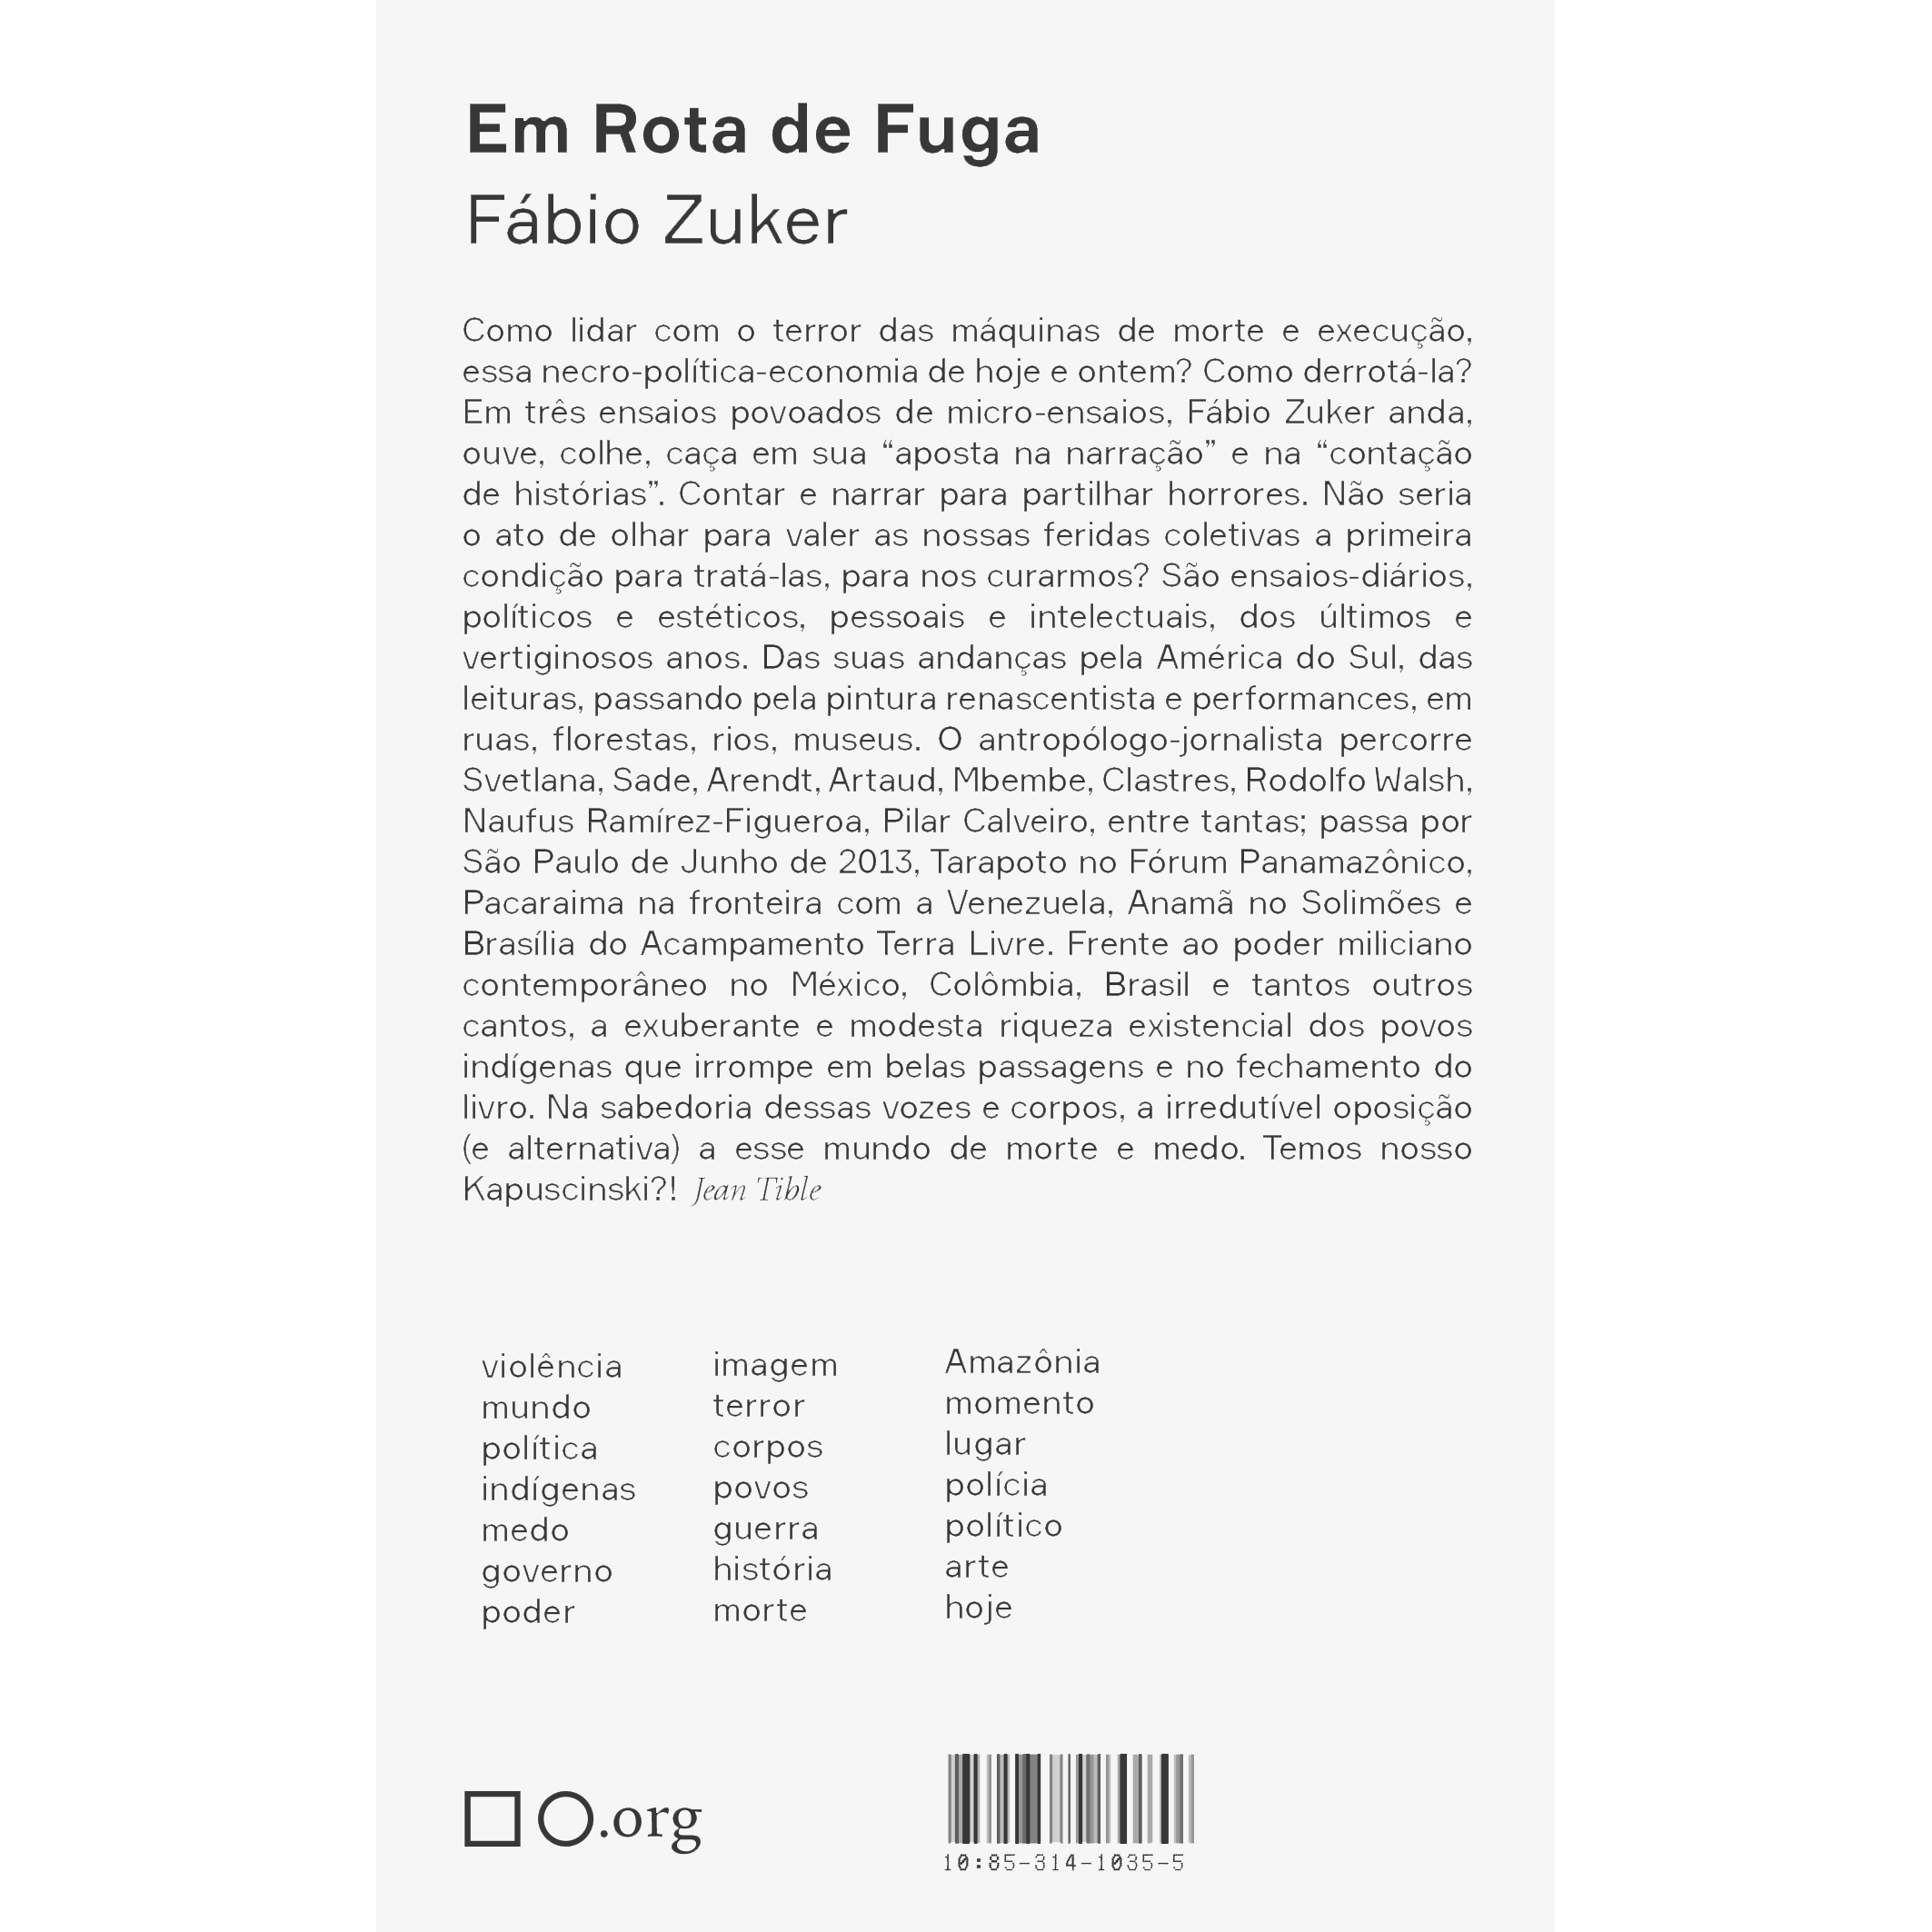
\includegraphics[width=92mm]{./grid/zuker.jpg}
\end{center}

\hspace*{-7cm}\hrulefill\hspace*{-7cm}

\medskip

\noindent{}O medo, em faceta promíscua aos mecanismos do governo neoliberal, é o fio condutor que percorre {\slsc{Em rota de fuga}}. Marcado por um olhar plurívoco, que perpassa a história da arte, Sade, cinema, vozes amazônicas e práticas de escrita contemporâneas, o escritor e antropólogo Fábio Zuker perscruta os desdobramentos dessa política para pensar outros mundos e formas de sensibilidade que criem efetivas rotas de fuga do círculo de violência neoliberal.

Ao tatear o “teatro"-peste” de Artaud enquanto político, analisar um quadro de Caravaggio ou abordar o medo do vazio que orientou o pensamento estético e político dos séculos passados, as reflexões do autor convergem para uma interrogação: a que servem as infinitas imagens de dor e violência diariamente veiculadas pela mídia? Como denunciar tais abusos e violências sem recorrer à megaexposição da morte, como fazem de forma quase ritualística as milícias latino"-americanas? A escrita surge enquanto potência disruptiva para questionar os moldes do poder e suas discursividades.

\vfill

\hspace*{-.4cm}\begin{minipage}[c]{.5\linewidth}
\small{
{\Formular{\textbf{
\hspace*{-.1cm}Título: Em rota de fuga – ensaios\\ sobre escrita, medo e violência\\
Autor: Fábio Zuker\\ 
ISBN: 978-85-7715-621-4\\
Páginas: 181\\
Formato: 11x18cm\\
Preço: R\$ 49,90\\
Editora: Quadradocirculo\\
Disponibilidade: 14/08/2020
}}}}
\end{minipage}


\pagebreak %SALTO NO ESCURO, TUCA VIEIRA

\begin{center}
\hspace*{.5cm}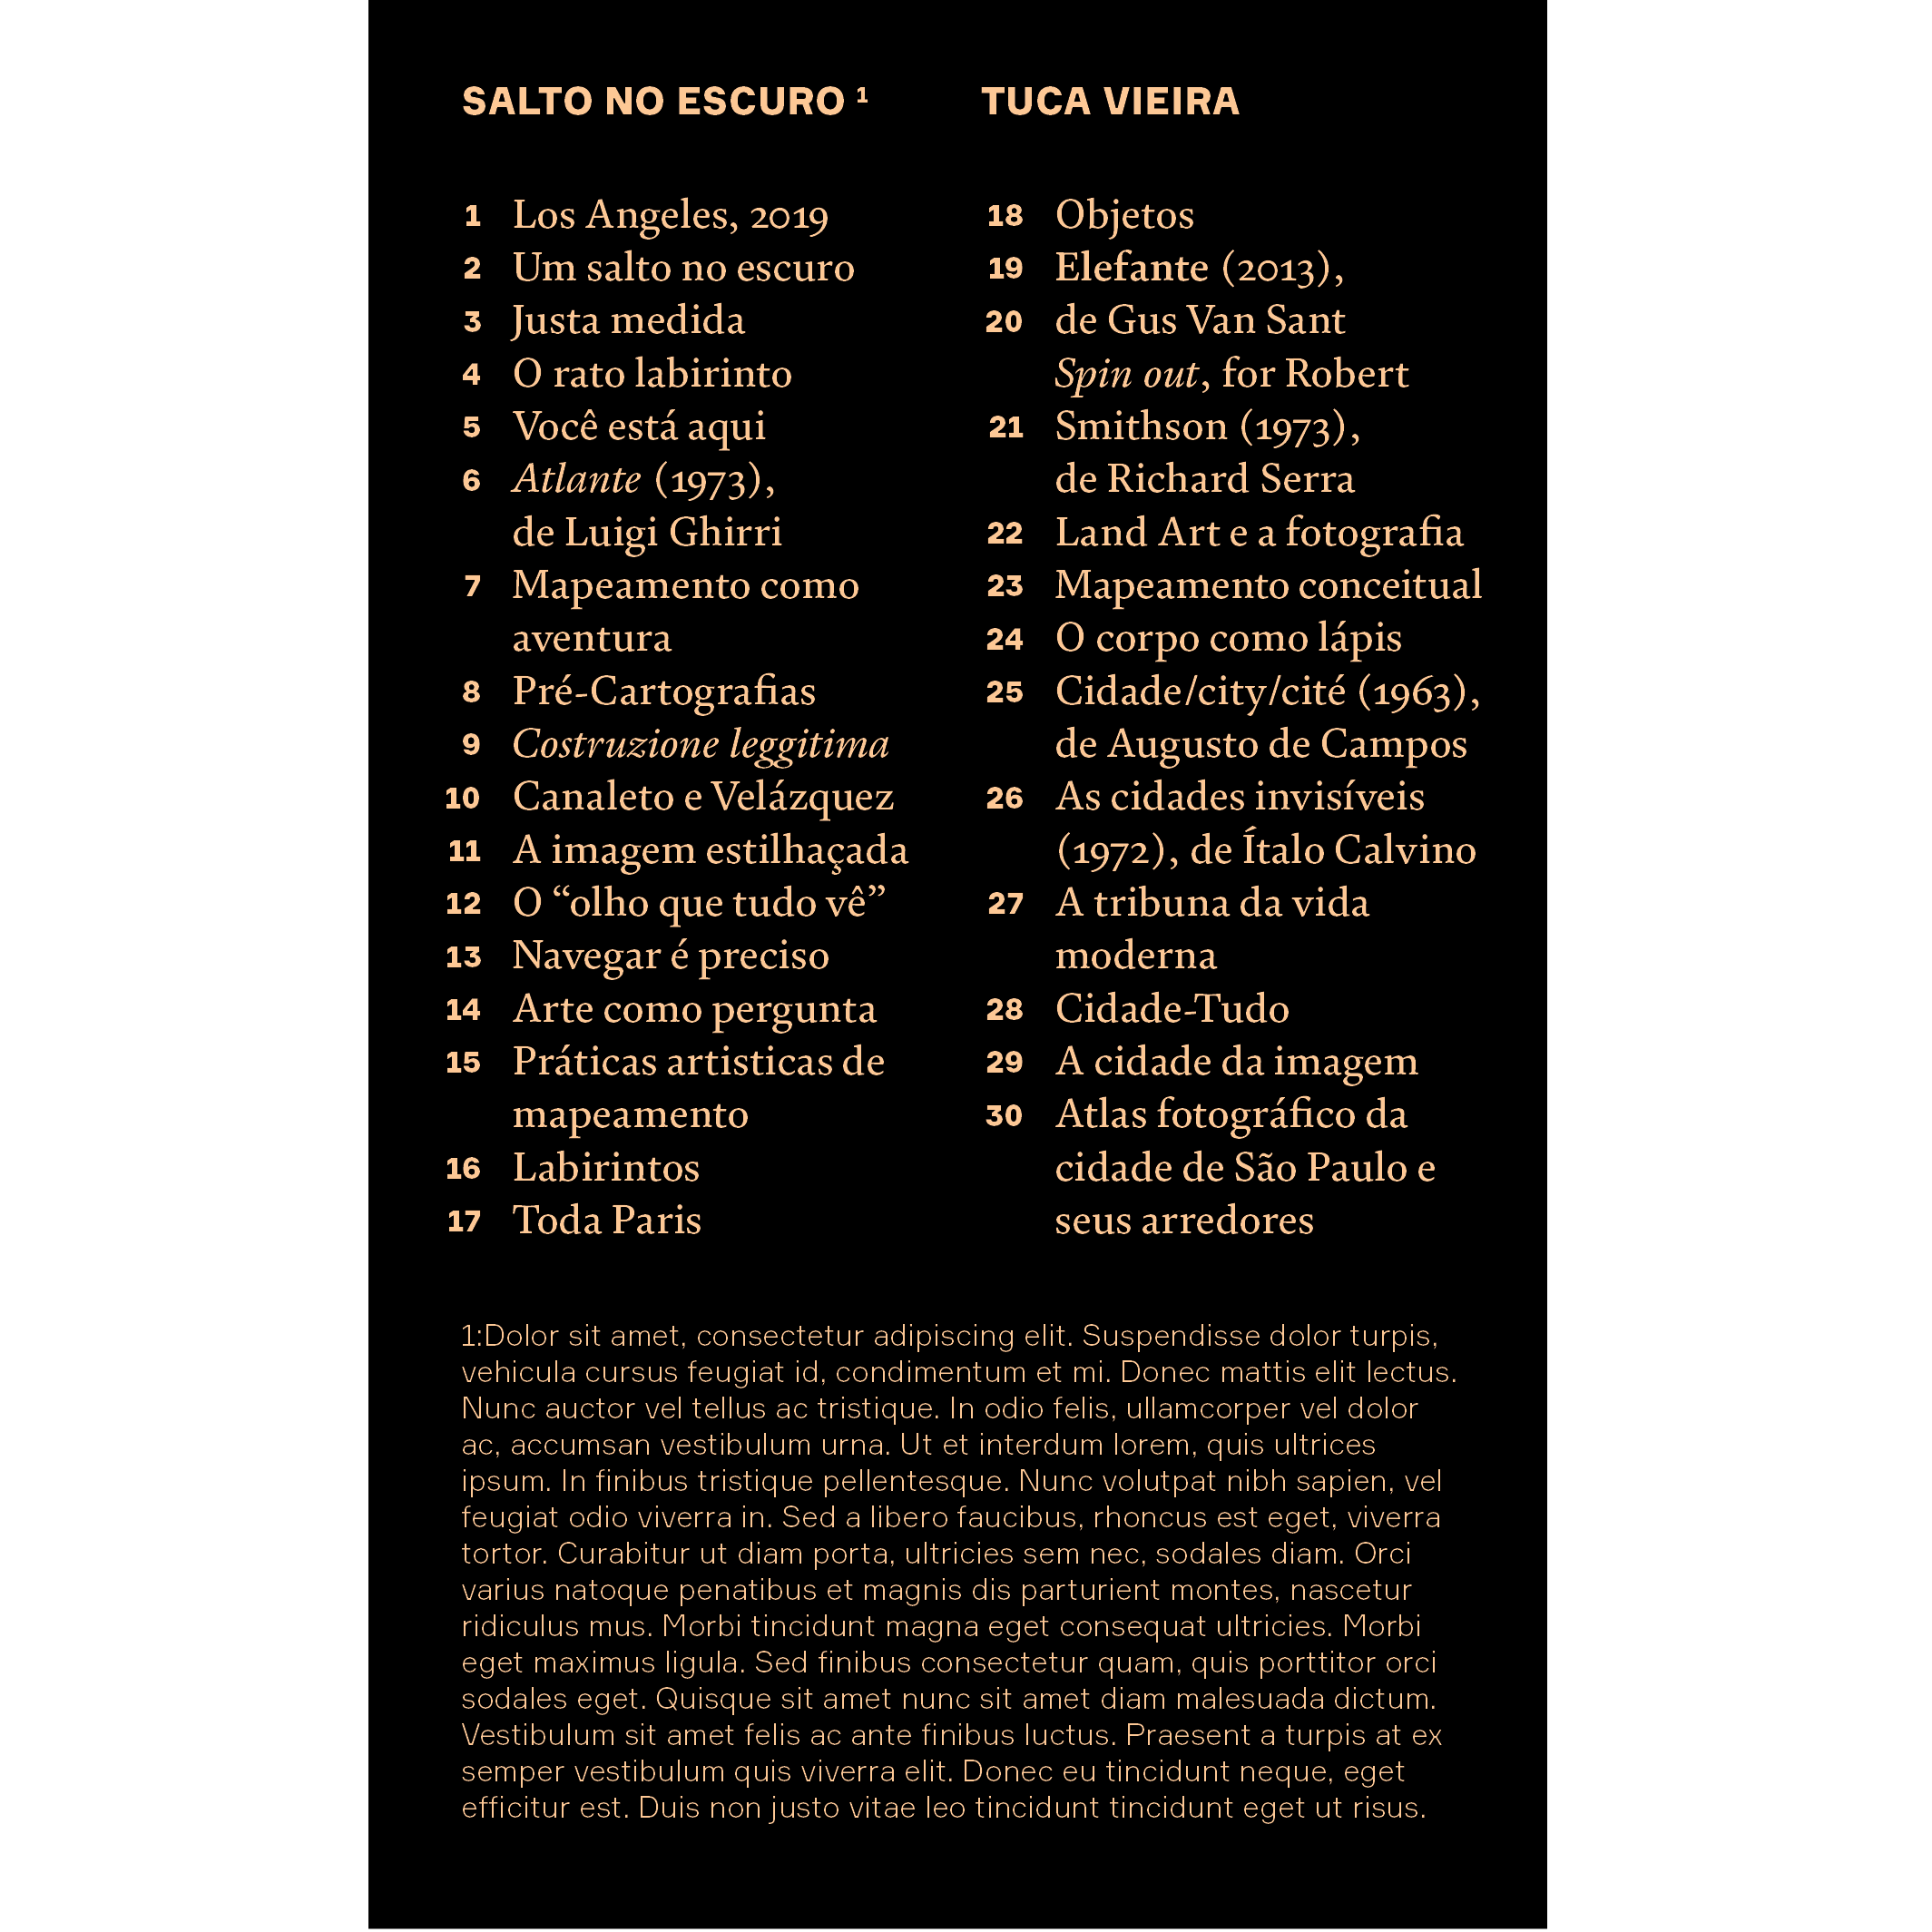
\includegraphics[width=92mm]{./grid/tuca.png}
\end{center}

\hspace*{-7cm}\hrulefill\hspace*{-7cm}

\medskip

\noindent{}Em um percurso que não deixa de ser um mapeamento afetivo do autor – com diversidade de referências literárias, cinematográficas, filosóficas, artísticas, históricas e arquitetônicas – {\slsc{Salto no escuro}} repensa criticamente as práticas de interação urbana, a partir de instigantes e assustadoras reflexões sobre as novas configurações espaciais das cidades.

O renomado fotógrafo Tuca Vieira frequenta os mais díspares e múltiplos caminhos, centros urbanos, labirintos e criações artísticas, munido de arcabouço teórico e filosófico para análises precisas e necessárias sobre a cidade contemporânea e novas formas de interação humana. Diversas expressões artísticas se entrecruzam nesse percurso – de Borges, Kafka e Velázquez a William Gibson, os poetas concretistas e artistas da Land Art. Diante da vertiginosa aceleração da vida e inédita realidade impostas pela tecnologia, o autor instiga novas possibilidades e percepções diante de uma experiência progressivamente calculada e enquadrada virtualmente. 

\vfill

\hspace*{-.4cm}\begin{minipage}[c]{.5\linewidth}
\small{
{\Formular{\textbf{
\hspace*{-.1cm}Título: Salto no escuro\\
Autor: Tuca Vieira\\ 
ISBN: 978-85-7715-622-1\\
Páginas: 490\\
Formato: 11x18cm\\
Preço: R\$ 79,90\\
Editora: Quadradocirculo\\
Disponibilidade: 14/08/2020
}}}}
\end{minipage}

\pagebreak